%!TEX TS-program = xelatex
%!TEX options = -aux-directory=Debug -shell-escape -file-line-error -interaction=nonstopmode -halt-on-error -synctex=1 "%DOC%"
\documentclass{article}
\input{LaTeX-Submodule/template.tex}

% Additional packages & macros
\DeclareMathOperator{\arccot}{arccot}
\DeclareMathOperator{\arcsec}{arcsec}
\DeclareMathOperator{\arccsc}{arccsc}

% Header and footer
\newcommand{\docTitle}{Trigonometry}

\fancyhead[L]{\docTitle}
\fancyhead[R]{\leftmark}
\fancyfoot[C]{\thepage}

% Copyright
\usepackage[
    type={CC},
    modifier={by-nc-sa},
    version={4.0},
    imagewidth={5em},
]{doclicense}

\author{Tarang Janawalkar}
\date{}

\begin{document}
%
\begin{titlepage}
    \vspace*{\fill}
    \begin{center}
        \LARGE\textbf{\docTitle}\\[0.2in]
        \normalsize\textsc{Tarang Janawalkar}
    \end{center}
    \vspace*{\fill}
    \doclicenseThis
    \thispagestyle{empty}
\end{titlepage}
\newpage
%
\tableofcontents
\newpage
%
\renewcommand*{\arraystretch}{1.25}
\section{Definitions}
\subsection{Trigonometric Functions}
The trigonometric definitions below are derived from the following right
triangle construction.
\begin{figure}[H]
    \centering
    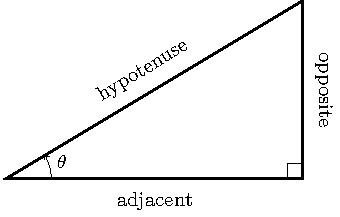
\includegraphics[height = 4cm, keepaspectratio = true]{figures/right-triangle.pdf}
\end{figure}
\begin{align*}
    \sin{\left( \theta \right)} & = \frac{\text{opposite}}{\text{hypotenuse}} & \csc{\left( \theta \right)} & = \frac{\text{hypotenuse}}{\text{opposite}} \\
    \cos{\left( \theta \right)} & = \frac{\text{adjacent}}{\text{hypotenuse}} & \sec{\left( \theta \right)} & = \frac{\text{hypotenuse}}{\text{adjacent}} \\
    \tan{\left( \theta \right)} & = \frac{\text{opposite}}{\text{adjacent}}   & \cot{\left( \theta \right)} & = \frac{\text{adjacent}}{\text{opposite}}
\end{align*}
\subsection{Inverse Trigonometric Functions}
\begin{align*}
    y = \arccos{\left( x \right)} & \iff x = \cos{\left( y \right)} & y = \arccsc{\left( x \right)} & \iff x = \csc{\left( y \right)} \\
    y = \arcsin{\left( x \right)} & \iff x = \sin{\left( y \right)} & y = \arcsec{\left( x \right)} & \iff x = \sec{\left( y \right)} \\
    y = \arctan{\left( x \right)} & \iff x = \tan{\left( y \right)} & y = \arccot{\left( x \right)} & \iff x = \cot{\left( y \right)}
\end{align*}
\subsection{Properties as a Real Function}
Let \(n\in\mathbb{Z}\) be a constant.
\begin{table}[H]
    \centering
    \begin{tabular}{c|cc|cc}
        \toprule
        \textbf{Function}          & \textbf{Period} & \textbf{Parity} & \textbf{Domain}                                                           & \textbf{Range}                                         \\
        \midrule
        \(\sin{\left( x \right)}\) & \(2\pi\)        & odd             & \(\mathbb{R}\)                                                            & \(\interval{-1}{1}\)                                   \\
        \(\cos{\left( x \right)}\) & \(2\pi\)        & even            & \(\mathbb{R}\)                                                            & \(\interval{-1}{1}\)                                   \\
        \(\tan{\left( x \right)}\) & \(\pi\)         & odd             & \(\mathbb{R}\backslash\Bigl\{ \left( n + \frac{1}{2} \right)\pi \Bigr\}\) & \(\mathbb{R}\)                                         \\
        \(\cot{\left( x \right)}\) & \(\pi\)         & odd             & \(\mathbb{R}\backslash\Bigl\{ n\pi \Bigr\}\)                              & \(\mathbb{R}\)                                         \\
        \(\sec{\left( x \right)}\) & \(2\pi\)        & even            & \(\mathbb{R}\backslash\Bigl\{ \left( n + \frac{1}{2} \right)\pi \Bigr\}\) & \(\linterval{-\infty}{-1} \cup \rinterval{1}{\infty}\) \\
        \(\csc{\left( x \right)}\) & \(2\pi\)        & odd             & \(\mathbb{R}\backslash\Bigl\{ n\pi \Bigr\}\)                              & \(\linterval{-\infty}{-1} \cup \rinterval{1}{\infty}\) \\
        \bottomrule
    \end{tabular}
\end{table}
\begin{table}[H]
    \centering
    \begin{tabular}{c|c|cc}
        \toprule
        \textbf{Function}             & \textbf{Parity} & \textbf{Domain}                                        & \textbf{Range}                                                             \\
        \midrule
        \(\arcsin{\left( x \right)}\) & odd             & \(\interval{-1}{1}\)                                   & \(\interval{-\frac{\pi}{2}}{\frac{\pi}{2}}\)                               \\
        \(\arccos{\left( x \right)}\) & --              & \(\interval{-1}{1}\)                                   & \(\interval{0}{\pi}\)                                                      \\
        \(\arctan{\left( x \right)}\) & odd             & \(\mathbb{R}\)                                         & \(\interval{-\frac{\pi}{2}}{\frac{\pi}{2}}\)                               \\
        \(\arccot{\left( x \right)}\) & odd             & \(\mathbb{R}\)                                         & \(\interval{0}{\pi}\)                                                      \\
        \(\arcsec{\left( x \right)}\) & --              & \(\linterval{-\infty}{-1} \cup \rinterval{1}{\infty}\) & \(\interval{0}{\pi} \backslash \left\{ \frac{\pi}{2} \right\}\)            \\
        \(\arccsc{\left( x \right)}\) & odd             & \(\linterval{-\infty}{-1} \cup \rinterval{1}{\infty}\) & \(\interval{-\frac{\pi}{2}}{\frac{\pi}{2}} \backslash \left\{ 0 \right\}\) \\
        \bottomrule
    \end{tabular}
\end{table}
\subsection{Symmetry}
\begin{align*}
    \sin{\left( -x \right)} & = -\sin{\left( x \right)} & \csc{\left( -x \right)} & = -\csc{\left( x \right)} \\
    \cos{\left( -x \right)} & =  \cos{\left( x \right)} & \sec{\left( -x \right)} & =  \sec{\left( x \right)} \\
    \tan{\left( -x \right)} & = -\tan{\left( x \right)} & \cot{\left( -x \right)} & = -\cot{\left( x \right)}
\end{align*}
\subsection{Periodicity}
Let \(n\in\mathbb{Z}\) be a constant.
\begin{align*}
    \sin{\left( x+2\pi n \right)} & = \sin{\left( x \right)} & \csc{\left( x+2\pi n \right)} & = \csc{\left( x \right)} \\
    \cos{\left( x+2\pi n \right)} & = \cos{\left( x \right)} & \sec{\left( x+2\pi n \right)} & = \sec{\left( x \right)} \\
    \tan{\left( x+\pi n \right)}  & = \tan{\left( x \right)} & \cot{\left( x+\pi n \right)}  & = \cot{\left( x \right)}
\end{align*}
\section{Trigonometric Identities}
\subsection{Pythagorean Identities}
\begin{equation*}
    \sin^2{\left( x \right)} + \cos^2{\left( x \right)} = 1
\end{equation*}
Dividing by either the sine or cosine function gives:
\begin{align*}
    \tan^2{\left( x \right)} + 1 & = \sec^2{\left( x \right)} \\
    1 + \cot^2{\left( x \right)} & = \csc^2{\left( x \right)}
\end{align*}
\subsection{Angle Sum Identities}
\begin{align*}
    \sin{\left( x\pm y \right)} & = \sin{\left( x \right)} \cos{\left( y \right)} \pm \cos{\left( x \right)} \sin{\left( y \right)}           & \csc{\left( x\pm y \right)} & = \frac{1}{\sin{\left( x \right)} \cos{\left( y \right)} \pm \cos{\left( x \right)} \sin{\left( y \right)}} \\
    \cos{\left( x\pm y \right)} & = \cos{\left( x \right)} \cos{\left( y \right)} \mp \sin{\left( x \right)} \sin{\left( y \right)}           & \sec{\left( x\pm y \right)} & = \frac{1}{\cos{\left( x \right)} \cos{\left( y \right)} \mp \sin{\left( x \right)} \sin{\left( y \right)}} \\
    \tan{\left( x\pm y \right)} & = \frac{\tan{\left( x \right)}\pm\tan{\left( y \right)}}{1\mp \tan{\left( x \right)}\tan{\left( y \right)}} & \cot{\left( x\pm y \right)} & = \frac{\cot{\left( x \right)}\cot{\left( y \right)}\mp 1}{\cot{\left( x \right)}\pm\cot{\left( y \right)}}
\end{align*}
\subsection{Double-Angle Identities}
\begin{align*}
    \sin{\left( 2x \right)} & = 2\sin{\left( x \right)}\cos{\left( x \right)}              & \csc{\left( 2x \right)} & = \frac{\sec{\left( x \right)}\csc{\left( x \right)}}{2}                                                     \\
    \cos{\left( 2x \right)} & = \cos^2{\left( x \right)} - \sin^2{\left( x \right)}        & \sec{\left( 2x \right)} & = \frac{\sec^2{\left( x \right)}\csc^2{\left( x \right)}}{\csc^2{\left( x \right)}-\sec^2{\left( x \right)}} \\
    \tan{\left( 2x \right)} & = \frac{2\tan{\left( x \right)}}{1-\tan^2{\left( x \right)}} & \cot{\left( 2x \right)} & = \frac{\cot^2{\left( x \right)}-1}{2\cot{\left( x \right)}}
\end{align*}
\subsection{Power Reducing Identities}
\begin{align*}
    \sin^2{\left( x \right)} & = \frac{1-\cos{\left( 2x \right)}}{2}                         & \csc^2{\left( x \right)} & = \frac{2}{1-\cos{\left( 2x \right)}}                         \\
    \cos^2{\left( x \right)} & = \frac{1+\cos{\left( 2x \right)}}{2}                         & \sec^2{\left( x \right)} & = \frac{2}{1+\cos{\left( 2x \right)}}                         \\
    \tan^2{\left( x \right)} & = \frac{1-\cos{\left( 2x \right)}}{1+\cos{\left( 2x \right)}} & \cot^2{\left( x \right)} & = \frac{1+\cos{\left( 2x \right)}}{1-\cos{\left( 2x \right)}}
\end{align*}
\subsection{Half Angle Identities}
\begin{align*}
    \sin{\left( \frac{x}{2} \right)} & = \left( -1 \right)^{\floor{\frac{x}{2\pi}}}\sqrt{\frac{1-\cos{\left( x \right)}}{2}}     & \csc{\left( \frac{x}{2} \right)} & = \left( -1 \right)^{\floor{\frac{x}{2\pi}}} \sqrt{\frac{2\sec{\left( x \right)}}{\sec{\left( x \right)}-1}}     \\
    \cos{\left( \frac{x}{2} \right)} & = \left( -1 \right)^{\floor{\frac{x+\pi}{2\pi}}}\sqrt{\frac{1+\cos{\left( x \right)}}{2}} & \sec{\left( \frac{x}{2} \right)} & = \left( -1 \right)^{\floor{\frac{x+\pi}{2\pi}}} \sqrt{\frac{2\sec{\left( x \right)}}{\sec{\left( x \right)}+1}} \\
    \tan{\left( \frac{x}{2} \right)} & = \frac{1-\cos{\left( x \right)}}{\sin{\left( x \right)}}                                 & \cot{\left( \frac{x}{2} \right)} & = \frac{\sin{\left( x \right)}}{1-\cos{\left( x \right)}}
\end{align*}
\subsection{Werner Identities}
\begin{align*}
    2\sin{\left( x \right)}\sin{\left( y \right)}  & = \cos{\left( x-y \right)}-\cos{\left( x+y \right)} \\
    2\cos{\left( x \right)}\cos{\left( y \right)}  & = \cos{\left( x-y \right)}+\cos{\left( x+y \right)} \\
    2\sin{\left( x \right)}\cos{\left( y \right)}  & = \sin{\left( x-y \right)}+\sin{\left( x+y \right)} \\
    -2\cos{\left( x \right)}\sin{\left( y \right)} & = \sin{\left( x-y \right)}-\sin{\left( x+y \right)}
\end{align*}
\subsection{Prosthaphaeresis Identities}
\begin{align*}
    \sin{\left( x \right)}+\sin{\left( y \right)} & = 2\sin{\left(\frac{x+y}{2} \right)}\cos{\left( \frac{x-y}{2} \right)}  \\
    \sin{\left( x \right)}-\sin{\left( y \right)} & = 2\cos{\left(\frac{x+y}{2} \right)}\sin{\left( \frac{x-y}{2} \right)}  \\
    \cos{\left( x \right)}+\cos{\left( y \right)} & = 2\cos{\left(\frac{x+y}{2} \right)}\cos{\left( \frac{x-y}{2} \right)}  \\
    \cos{\left( x \right)}-\cos{\left( y \right)} & = -2\sin{\left(\frac{x+y}{2} \right)}\sin{\left( \frac{x-y}{2} \right)} \\
\end{align*}
\subsection{Inverse Reciprocal Identities}
\begin{align*}
    \arcsin{\left( \frac{1}{x} \right)} & = \arccsc{\left( x \right)} & \arccsc{\left( \frac{1}{x} \right)} & = \arcsin{\left( x \right)} \\
    \arccos{\left( \frac{1}{x} \right)} & = \arcsec{\left( x \right)} & \arcsec{\left( \frac{1}{x} \right)} & = \arccos{\left( x \right)} \\
    \arctan{\left( \frac{1}{x} \right)} & = \arccot{\left( x \right)} & \arccot{\left( \frac{1}{x} \right)} & = \arctan{\left( x \right)} \\
\end{align*}
\section{Geometric Identities}
\begin{figure}[H]
    \centering
    \includegraphics*{figures/triangle.pdf}
\end{figure}
\subsection{Area of a Triangle}
\begin{equation*}
    A=\frac{1}{2}a b \sin{\left( \gamma \right)}
\end{equation*}
\subsection{Sine Rule}
\begin{equation*}
    \frac{\sin{\left( \alpha \right)}}{a} = \frac{\sin{\left( \beta \right)}}{b} = \frac{\sin{\left( \gamma \right)}}{c}
\end{equation*}
\subsection{Cosine Rule}
\begin{equation*}
    a^2=b^2+c^2-2b c\cos{\left( \alpha \right)}
\end{equation*}
\subsection{Tangent Rule}
\begin{equation*}
    \frac{\tan{\left( \frac{\alpha-\beta}{2} \right)}}{\tan{\left( \frac{\alpha+\beta}{2} \right)}} = \frac{a-b}{a+b}
\end{equation*}
\subsection{Mollweide's Identity}
\begin{equation*}
    \frac{b-c}{a}=\frac{\sin{\left( \frac{\beta-\gamma}{2} \right)}}{\cos{\left( \frac{\alpha}{2} \right)}}
\end{equation*}
\subsection{Newton's Identity}
\begin{equation*}
    \frac{b+c}{a}=\frac{\cos{\left( \frac{\beta-\gamma}{2} \right)}}{\sin{\left( \frac{\alpha}{2} \right)}}
\end{equation*}
\section{The Unit Circle}
The unit circle \(C\) is defined as the set of all points \(\left( x,\: y \right)\)
which satisfy the equation
\begin{equation*}
    x^2 + y^2 = 1,
\end{equation*}
or, mathematically,
\begin{equation*}
    C = \left\{ \left( x,\: y \right) \,\vert\, x^2 + y^2 = 1 \right\}.
\end{equation*}
A graph of this function is shown below.
\begin{figure}[H]
    \centering
    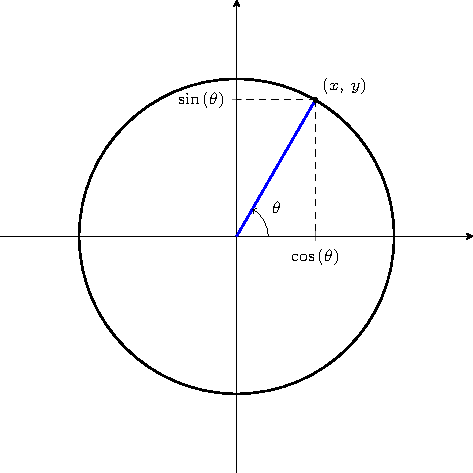
\includegraphics[width=8cm]{figures/unit-circle.pdf}
\end{figure}
A point that lies on this circle can be described by the angle it forms
with the positive \(x\)-axis. This point has the components:
\begin{equation*}
    \left( x,\: y \right) = \left( \cos{\left( \theta \right)},\: \sin{\left( \theta \right)} \right).
\end{equation*}
\subsection{Special Triangles}
The following right triangle constructions provide coordinates of
points that form an angle of \(\pi/6\), \(\pi/4\), or \(\pi/3\) from the
positive \(x\)-axis.
\begin{figure}[H]
    \centering
    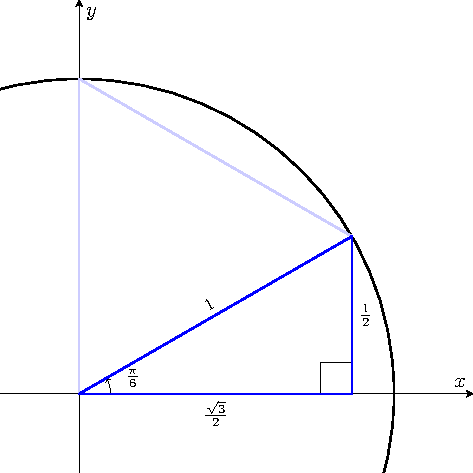
\includegraphics[width=8cm]{figures/unit-circle-30.pdf}
\end{figure}
\begin{figure}[H]
    \centering
    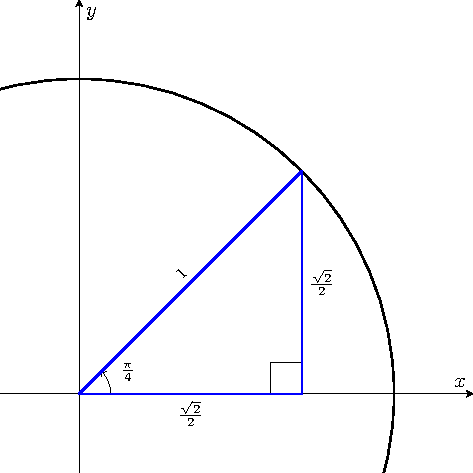
\includegraphics[width=8cm]{figures/unit-circle-45.pdf}
\end{figure}
\begin{figure}[H]
    \centering
    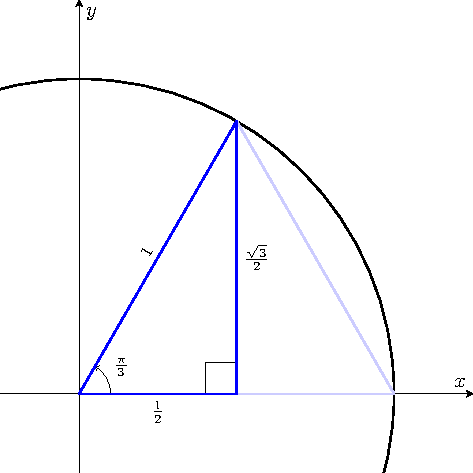
\includegraphics[width=8cm]{figures/unit-circle-60.pdf}
\end{figure}
This is summarised in the table below.
\begin{table}[H]
    \centering
    \begin{tabular}{c c c}
        \toprule
        \textbf{Angle from Positive \(x\)-axis} & \textbf{Horizontal Component}                  & \textbf{Vertical Component}                    \\
        \midrule
        \(\displaystyle\frac{\pi}{6} = 30^\circ\) & \(\displaystyle\frac{\sqrt{3}}{2} \approx \num{0.866025}\) & \(\displaystyle\frac{1}{2} = 0.5\)                         \\[2ex]
        \(\displaystyle\frac{\pi}{4} = 45^\circ\) & \(\displaystyle\frac{\sqrt{2}}{2} \approx \num{0.707107}\) & \(\displaystyle\frac{\sqrt{2}}{2} \approx \num{0.707107}\) \\[2ex]
        \(\displaystyle\frac{\pi}{6} = 30^\circ\) & \(\displaystyle\frac{1}{2} = 0.5\)                         & \(\displaystyle\frac{\sqrt{3}}{2} \approx \num{0.866025}\) \\[2ex]
        \bottomrule
    \end{tabular}
    % \caption{} % \label{}
\end{table}
\subsection{2-Argument Arctangent}
Consider a point \(\left( x,\: y \right)\) that lies on the Cartesian
plane. The angle measure from the positive \(x\)-axis and the ray from
the origin to the point \(\left( x,\: y \right)\) is defined by the
2-argument arctangent function:
\begin{equation*}
    \operatorname{atan2}\left( y,\: x \right) =
    \begin{cases}
        \arctan{\left( \frac{y}{x} \right)}       & \text{if \(x > 0\)},                       \\
        \arctan{\left( \frac{y}{x} \right)} + \pi & \text{if \(x < 0\) and \(y \geqslant 0\)}, \\
        \arctan{\left( \frac{y}{x} \right)} - \pi & \text{if \(x < 0\) and \(y < 0\)},         \\
        +\frac{\pi}{2}                            & \text{if \(x = 0\) and \(y > 0\)},         \\
        -\frac{\pi}{2}                            & \text{if \(x = 0\) and \(y < 0\)},         \\
        \text{undefined}                          & \text{if \(x = 0\) and \(y = 0\)}.
    \end{cases}
\end{equation*}
This definition allows an angle measure to be obtained in any quadrant
of the Cartesian plane, on the interval \(\linterval{-\pi}{\pi}\).
When \(x\) and \(y\) describe the real and imaginary parts of a complex
number \(z = x + yi\), the 2-argument arctangent is precisely the
principal argument of \(z\):
\begin{equation*}
    \operatorname{Arg}\left( z \right) = \operatorname{atan2}\left( y,\: x \right),
\end{equation*}
defined on the same interval \(\linterval{-\pi}{\pi}\).
Note that the set of all arguments of a complex number is defined by the
general argument:
\begin{equation*}
    \arg{\left( z \right)} = \left\{ \operatorname{Arg}\left( z \right) + 2\pi n \,\vert\, n \in \Z \right\}.
\end{equation*}
These angles can be geometrically determined by considering the quadrant
in which the point lies.
\begin{figure}[H]
    \centering
    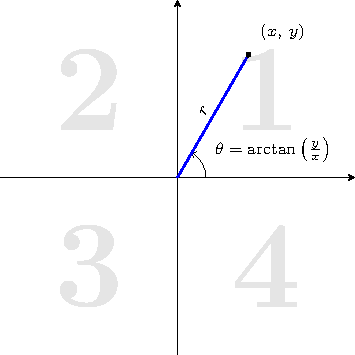
\includegraphics[width=8cm]{figures/Arg-q1.pdf}
\end{figure}
\begin{figure}[H]
    \centering
    \includegraphics[width=8cm]{figures/Arg-q2.pdf}
\end{figure}
\begin{figure}[H]
    \centering
    \includegraphics[width=8cm]{figures/Arg-q3.pdf}
\end{figure}
\begin{figure}[H]
    \centering
    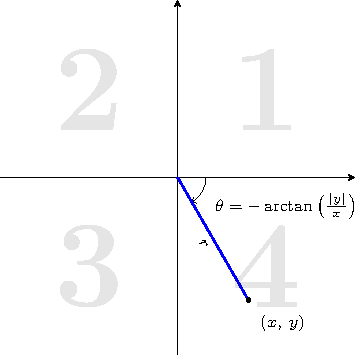
\includegraphics[width=8cm]{figures/Arg-q4.pdf}
\end{figure}
This is summarised below.
\begin{table}[H]
    \centering
    \begin{tabular}{c c c c}
        \toprule
        \textbf{Quadrant} & \textbf{Sign} \(x\) & \textbf{Sign} \(y\) & \textbf{Angle Measure} \(\theta\)                      \\
        \midrule
        First             & \({}+{}\)           & \({}+{}\)           & \(\arctan{\left( \frac{y}{x} \right)}\)                \\
        Second            & \({}-{}\)           & \({}+{}\)           & \(\pi - \arctan{\left( \frac{y}{\abs*{x}} \right)}\)   \\
        Third             & \({}-{}\)           & \({}-{}\)           & \(-\pi + \arctan{\left( \frac{\abs*{y}}{x} \right)}\)  \\
        Fourth            & \({}+{}\)           & \({}-{}\)           & \(-\arctan{\left( \frac{\abs*{y}}{\abs*{x}} \right)}\) \\
        \bottomrule
    \end{tabular}
    % \caption{} % \label{}
\end{table}
\end{document}
